\documentclass[main.tex]{subfiles}
\begin{document}

\begin{frame}
\frametitle{Likelihood}

Suppose that we have a list of speeds for a single animal over time: $S:=\{S_t\}_{t=1}^T$.

\vspace{0.5cm}

If we knew the states, $X:=\{X_t\}_{t=1}^T$, since $S_t | X_t \overset{\text{iid}}{\sim} \text{normal}(\mu_{x_t}, \sigma_{x_t})$


the likelihood takes the form:
%
\begin{equation}
    p(S|X,\theta) = \prod_{t=1}^T p(S_t | X_t, \theta).
\end{equation}

But we don't know the states. So what do we do?
    
\end{frame}

\begin{frame}
\frametitle{The joint density of speeds and states}

We consider instead the joint density (suppressing $\theta$ dependence from now on):
%
\begin{equation}
    \begin{aligned}
    p(S, X) &= p(S|X) \times p(X)\\
    &= \left[\prod_{t=1}^T p(S_t | X_t)\right] \times p(X_t)\\
    &= \left[\prod_{t=1}^T p(S_t | X_t)\right] \times \left[\prod_{t=2}^T p(X_t | X_{t-1})\right] p(X_1)
    \end{aligned}
\end{equation}
    
\end{frame}

\begin{frame}
\frametitle{Likelihood revisited}

We can obtain the likelihood by marginalising out $X$ from our joint:
%
\begin{equation}
    p(S) = \sum_X p(S,X).
\end{equation}
%
What does this mean?

\end{frame}

\begin{frame}
\frametitle{Marginalising out variables of joint distributions}

		
\begin{figure}[ht]
    \centerline{\includegraphics[width=0.6\textwidth]{./figures/horse_race_marginal.pdf}}
\end{figure}
    
\end{frame}

\begin{frame}
\frametitle{Likelihood revisited}

\begin{equation}
    p(S) = \sum_X p(S,X).
\end{equation}

But this really means:
%
\begin{equation}
    p(S) = \sum_{X_1}\sum_{X_2}...\sum_{X_T}\left[\prod_{t=1}^T p(S_t | X_t)\right] \times \left[\prod_{t=2}^T p(X_t | X_{t-1})\right] p(X_1).
\end{equation}
%
So the computational expense scales as $N^T$, where $N$ is number of states!
    
\end{frame}

\begin{frame}
\frametitle{The forward algorithm: a much cheaper way to evaluate the likelihood}

The \textit{forward algorithm} is an approach from dynamic programming which stores intermediate probabilities.

\vspace{0.5cm}

It uses a marginalisation trick to calculate the likelihood:

\begin{equation}
    \begin{aligned}
    p(S_1, S_2, ..., S_T) = \sum_{i=1}^N p(S_1, S_2, ..., S_T, X_T=j).
    \end{aligned}
\end{equation}

\vspace{0.5cm}

But how do we calculate the RHS?
    
\end{frame}

\begin{frame}
\frametitle{Forward algorithm bookkeeping}

Consider again the joint distribution of the observations and the final state:

\begin{equation}
    \begin{aligned}
    \textcolor{orange}{p(S_1, S_2, ..., }&\textcolor{orange}{S_T, X_T=j)} = p(S_T | X_T = j) \times\\ &\sum_{i=1}^N p(X_T=j | X_{T-1}=i) \times \textcolor{blue}{p(S_1, S_2, ..., S_{T-1}, X_{T-1}=i)}
    \end{aligned}
\end{equation}

which looks like:

\begin{equation}
    \begin{aligned}
    \textcolor{orange}{\alpha_t(j)} = p(S_T | X_T = j) \times\sum_{i=1}^N p(X_T=j | X_{T-1}=i) \times \textcolor{blue}{\alpha_{t-1}(j)},
    \end{aligned}
\end{equation}

with $\alpha_1(j)=p(S_1 | X_1 = j)p(X_1=j)$.
    
\end{frame}

\begin{frame}
\frametitle{Incremental calculation of likelihood}


\begin{center}
\begin{tikzpicture}[node distance=2cm, block/.style={draw, minimum width=1cm, minimum height=1cm}]

  % First row
  \node[block] (A1) {$\alpha_1(m)$};
  \node[block, right of=A1] (A2) {};
  \node[block, right of=A2] (A3) {};
  \node[block, right of=A3] (A4) {};

  % Second row
  \node[block, below of=A1] (B1) {};
  \node[block, right of=B1] (B2) {};
  \node[block, right of=B2] (B3) {};
  \node[block, right of=B3] (B4) {};

  % Labels
  \node[coordinate, left of=A1] (J1) {};
  \node[] at (J1) {Migrating:};
  \node[coordinate, left of=B1] (J2) {};
  \node[] at (J2) {Foraging:};

  \node[coordinate, above of=A1, yshift=-1.25cm] (G1) {};
  \node[above] at (G1) {$S_1$};
  \node[coordinate, above of=A2, yshift=-1.25cm] (G2) {};
  \node[above] at (G2) {};
  \node[coordinate, above of=A3, yshift=-1.25cm] (G3) {};
  \node[above] at (G3) {};
  \node[coordinate, above of=A4, yshift=-1.25cm] (G4) {};
  \node[above] at (G4) {};
  \node[coordinate, below of=B1, yshift=1.25cm] (H1) {};
  \node[below] at (H1) {};
  \node[coordinate, below of=B2, yshift=1.25cm] (H2) {};
  \node[below] at (H2) {};
  \node[coordinate, below of=B3, yshift=1.25cm] (H3) {};
  \node[below] at (H3) {};
  \node[coordinate, below of=B4, yshift=1.25cm] (H4) {};
  \node[below] at (H4) {};

  % vertical arrow
  \draw[->, line width=1pt, opacity=1, color=purple] (A1.north) -- (G1.south);

  % Horizontal arrows
  \draw[->, line width=1pt, opacity=0] (A1.east) -- (A2.west);
  \draw[->, line width=1pt, opacity=0] (A2.east) -- (A3.west);
  \draw[->, line width=1pt, opacity=0] (A3.east) -- (A4.west);
  \draw[->, line width=1pt, opacity=0] (B1.east) -- (B2.west);
  \draw[->, line width=1pt, opacity=0] (B2.east) -- (B3.west);
  \draw[->, line width=1pt, opacity=0] (B3.east) -- (B4.west);

  % diagonal to blocks
  \draw[->, line width=1pt, opacity=0] (A1.south east) -- (B2.north);
  \draw[->, line width=1pt, opacity=0] (A2.south east) -- (B3.north);
  \draw[->, line width=1pt, opacity=0] (A3.south east) -- (B4.north);
  \draw[->, line width=1pt, opacity=0] (B1.north east) -- (A2.south);
  \draw[->, line width=1pt, opacity=0] (B2.north east) -- (A3.south);
  \draw[->, line width=1pt, opacity=0] (B3.north east) -- (A4.south);

\end{tikzpicture}
\end{center}

where $\alpha_1(m)=\textcolor{purple}{p(S_1 | X_1 = m)p(X_1=m)}$.
    
\end{frame}

\begin{frame}
\frametitle{Incremental calculation of likelihood}


\begin{center}
\begin{tikzpicture}[node distance=2cm, block/.style={draw, minimum width=1cm, minimum height=1cm}]

  % First row
  \node[block] (A1) {$\alpha_1(m)$};
  \node[block, right of=A1] (A2) {};
  \node[block, right of=A2] (A3) {};
  \node[block, right of=A3] (A4) {};

  % Second row
  \node[block, below of=A1] (B1) {$\alpha_1(f)$};
  \node[block, right of=B1] (B2) {};
  \node[block, right of=B2] (B3) {};
  \node[block, right of=B3] (B4) {};

  % Labels
  \node[coordinate, left of=A1] (J1) {};
  \node[] at (J1) {Migrating:};
  \node[coordinate, left of=B1] (J2) {};
  \node[] at (J2) {Foraging:};

  \node[coordinate, above of=A1, yshift=-1.25cm] (G1) {};
  \node[above] at (G1) {};
  \node[coordinate, above of=A2, yshift=-1.25cm] (G2) {};
  \node[above] at (G2) {};
  \node[coordinate, above of=A3, yshift=-1.25cm] (G3) {};
  \node[above] at (G3) {};
  \node[coordinate, above of=A4, yshift=-1.25cm] (G4) {};
  \node[above] at (G4) {};
  \node[coordinate, below of=B1, yshift=1.25cm] (H1) {};
  \node[below] at (H1) {$S_1$};
  \node[coordinate, below of=B2, yshift=1.25cm] (H2) {};
  \node[below] at (H2) {};
  \node[coordinate, below of=B3, yshift=1.25cm] (H3) {};
  \node[below] at (H3) {};
  \node[coordinate, below of=B4, yshift=1.25cm] (H4) {};
  \node[below] at (H4) {};

  % vertical arrow
  \draw[->, line width=1pt, opacity=1, color=purple] (B1.south) -- (H1.north);

  % Horizontal arrows
  \draw[->, line width=1pt, opacity=0] (A1.east) -- (A2.west);
  \draw[->, line width=1pt, opacity=0] (A2.east) -- (A3.west);
  \draw[->, line width=1pt, opacity=0] (A3.east) -- (A4.west);
  \draw[->, line width=1pt, opacity=0] (B1.east) -- (B2.west);
  \draw[->, line width=1pt, opacity=0] (B2.east) -- (B3.west);
  \draw[->, line width=1pt, opacity=0] (B3.east) -- (B4.west);

  % diagonal to blocks
  \draw[->, line width=1pt, opacity=0] (A1.south east) -- (B2.north);
  \draw[->, line width=1pt, opacity=0] (A2.south east) -- (B3.north);
  \draw[->, line width=1pt, opacity=0] (A3.south east) -- (B4.north);
  \draw[->, line width=1pt, opacity=0] (B1.north east) -- (A2.south);
  \draw[->, line width=1pt, opacity=0] (B2.north east) -- (A3.south);
  \draw[->, line width=1pt, opacity=0] (B3.north east) -- (A4.south);

\end{tikzpicture}
\end{center}

where $\alpha_1(f)=\textcolor{purple}{p(S_1 | X_1 = f)p(X_1=f)}$.
    
\end{frame}


\begin{frame}
\frametitle{Incremental calculation of likelihood}


\begin{center}
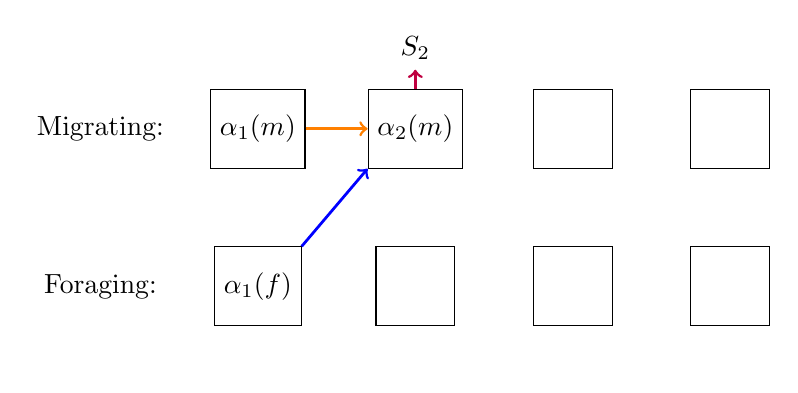
\begin{tikzpicture}[node distance=2cm, block/.style={draw, minimum width=1cm, minimum height=1cm}]

  % First row
  \node[block] (A1) {$\alpha_1(m)$};
  \node[block, right of=A1] (A2) {$\alpha_2(m)$};
  \node[block, right of=A2] (A3) {};
  \node[block, right of=A3] (A4) {};

  % Second row
  \node[block, below of=A1] (B1) {$\alpha_1(f)$};
  \node[block, right of=B1] (B2) {};
  \node[block, right of=B2] (B3) {};
  \node[block, right of=B3] (B4) {};

  % Labels
  \node[coordinate, left of=A1] (J1) {};
  \node[] at (J1) {Migrating:};
  \node[coordinate, left of=B1] (J2) {};
  \node[] at (J2) {Foraging:};

  \node[coordinate, above of=A1, yshift=-1.25cm] (G1) {};
  \node[above] at (G1) {};
  \node[coordinate, above of=A2, yshift=-1.25cm] (G2) {};
  \node[above] at (G2) {$S_2$};
  \node[coordinate, above of=A3, yshift=-1.25cm] (G3) {};
  \node[above] at (G3) {};
  \node[coordinate, above of=A4, yshift=-1.25cm] (G4) {};
  \node[above] at (G4) {};
  \node[coordinate, below of=B1, yshift=1.25cm] (H1) {};
  \node[below] at (H1) {};
  \node[coordinate, below of=B2, yshift=1.25cm] (H2) {};
  \node[below] at (H2) {};
  \node[coordinate, below of=B3, yshift=1.25cm] (H3) {};
  \node[below] at (H3) {};
  \node[coordinate, below of=B4, yshift=1.25cm] (H4) {};
  \node[below] at (H4) {};

  % Horizontal arrows
  \draw[->, line width=1pt, opacity=1, color=orange] (A1.east) -- (A2.west);
  \draw[->, line width=1pt, opacity=0] (A2.east) -- (A3.west);
  \draw[->, line width=1pt, opacity=0] (A3.east) -- (A4.west);
  \draw[->, line width=1pt, opacity=0] (B1.east) -- (B2.west);
  \draw[->, line width=1pt, opacity=0] (B2.east) -- (B3.west);
  \draw[->, line width=1pt, opacity=0] (B3.east) -- (B4.west);

  % diagonal to blocks
  \draw[->, line width=1pt, opacity=0] (A1.south east) -- (B2.north);
  \draw[->, line width=1pt, opacity=0] (A2.south east) -- (B3.north);
  \draw[->, line width=1pt, opacity=0] (A3.south east) -- (B4.north);
  \draw[->, line width=1pt, opacity=1,color=blue] (B1.north east) -- (A2.south west);
  \draw[->, line width=1pt, opacity=0] (B2.north east) -- (A3.south);
  \draw[->, line width=1pt, opacity=0] (B3.north east) -- (A4.south);

  % vertical arrow
  \draw[->, line width=1pt, opacity=1, color=purple] (A2.north) -- (G2.south);


\end{tikzpicture}
\end{center}

where: 
\begin{equation}
    \begin{aligned}
    \alpha_2(m) = &\{\textcolor{orange}{p(X_2=m | X_1=m) \alpha_{1}(m)} +\textcolor{blue}{p(X_2=m | X_1=f) \alpha_{1}(f)}\}\\
    &\times \textcolor{purple}{p(S_2 | X_2 = m)}.
    \end{aligned}
\end{equation}
    
\end{frame}

\begin{frame}
\frametitle{Incremental calculation of likelihood}


\begin{center}
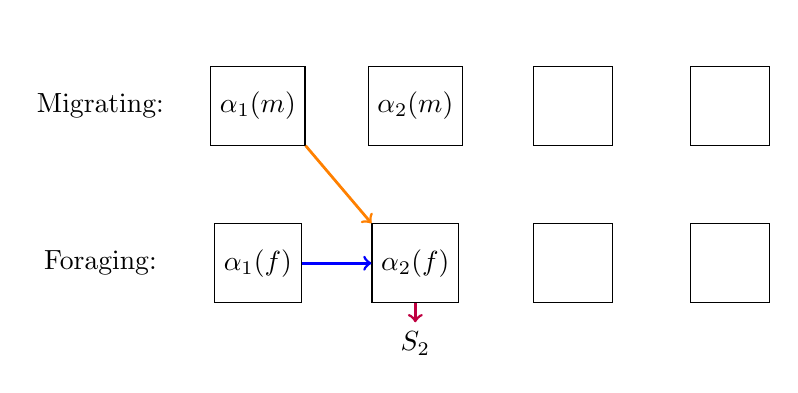
\begin{tikzpicture}[node distance=2cm, block/.style={draw, minimum width=1cm, minimum height=1cm}]

  % First row
  \node[block] (A1) {$\alpha_1(m)$};
  \node[block, right of=A1] (A2) {$\alpha_2(m)$};
  \node[block, right of=A2] (A3) {};
  \node[block, right of=A3] (A4) {};

  % Second row
  \node[block, below of=A1] (B1) {$\alpha_1(f)$};
  \node[block, right of=B1] (B2) {$\alpha_2(f)$};
  \node[block, right of=B2] (B3) {};
  \node[block, right of=B3] (B4) {};

  % Labels
  \node[coordinate, left of=A1] (J1) {};
  \node[] at (J1) {Migrating:};
  \node[coordinate, left of=B1] (J2) {};
  \node[] at (J2) {Foraging:};

  \node[coordinate, above of=A1, yshift=-1.25cm] (G1) {};
  \node[above] at (G1) {};
  \node[coordinate, above of=A2, yshift=-1.25cm] (G2) {};
  \node[above] at (G2) {};
  \node[coordinate, above of=A3, yshift=-1.25cm] (G3) {};
  \node[above] at (G3) {};
  \node[coordinate, above of=A4, yshift=-1.25cm] (G4) {};
  \node[above] at (G4) {};
  \node[coordinate, below of=B1, yshift=1.25cm] (H1) {};
  \node[below] at (H1) {};
  \node[coordinate, below of=B2, yshift=1.25cm] (H2) {};
  \node[below] at (H2) {$S_2$};
  \node[coordinate, below of=B3, yshift=1.25cm] (H3) {};
  \node[below] at (H3) {};
  \node[coordinate, below of=B4, yshift=1.25cm] (H4) {};
  \node[below] at (H4) {};

  % Horizontal arrows
  \draw[->, line width=1pt, opacity=0] (A1.east) -- (A2.west);
  \draw[->, line width=1pt, opacity=0] (A2.east) -- (A3.west);
  \draw[->, line width=1pt, opacity=0] (A3.east) -- (A4.west);
  \draw[->, line width=1pt, opacity=1,color=blue] (B1.east) -- (B2.west);
  \draw[->, line width=1pt, opacity=0] (B2.east) -- (B3.west);
  \draw[->, line width=1pt, opacity=0] (B3.east) -- (B4.west);

  % diagonal to blocks
  \draw[->, line width=1pt, opacity=1,color=orange] (A1.south east) -- (B2.north west);
  \draw[->, line width=1pt, opacity=0] (A2.south east) -- (B3.north);
  \draw[->, line width=1pt, opacity=0] (A3.south east) -- (B4.north);
  \draw[->, line width=1pt, opacity=0] (B1.north east) -- (A2.south west);
  \draw[->, line width=1pt, opacity=0] (B2.north east) -- (A3.south);
  \draw[->, line width=1pt, opacity=0] (B3.north east) -- (A4.south);

  % vertical arrow
  \draw[->, line width=1pt, opacity=1, color=purple] (B2.south) -- (H2.north);

\end{tikzpicture}
\end{center}

where: 
\begin{equation}
    \begin{aligned}
    \alpha_2(f) = \{&\textcolor{orange}{p(X_2=f | X_1=m) \alpha_{1}(m)} +\textcolor{blue}{p(X_2=f | X_1=f) \alpha_{1}(f)}\}\\
    &\times \textcolor{purple}{p(S_2| X_2 = f)} 
    \end{aligned}
\end{equation}
    
\end{frame}

\begin{frame}
\frametitle{Incremental calculation of likelihood}


\begin{center}
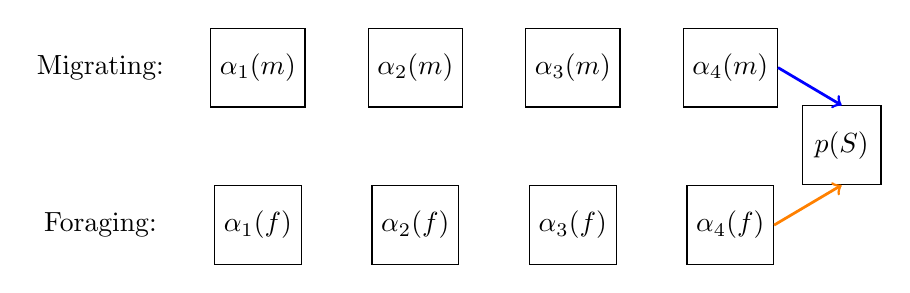
\begin{tikzpicture}[node distance=2cm, block/.style={draw, minimum width=1cm, minimum height=1cm}]

  % First row
  \node[block] (A1) {$\alpha_1(m)$};
  \node[block, right of=A1] (A2) {$\alpha_2(m)$};
  \node[block, right of=A2] (A3) {$\alpha_3(m)$};
  \node[block, right of=A3] (A4) {$\alpha_4(m)$};

  % Second row
  \node[block, below of=A1] (B1) {$\alpha_1(f)$};
  \node[block, right of=B1] (B2) {$\alpha_2(f)$};
  \node[block, right of=B2] (B3) {$\alpha_3(f)$};
  \node[block, right of=B3] (B4) {$\alpha_4(f)$};


  % Labels
  \node[coordinate, left of=A1] (J1) {};
  \node[] at (J1) {Migrating:};
  \node[coordinate, left of=B1] (J2) {};
  \node[] at (J2) {Foraging:};

  % Horizontal arrows
  \draw[->, line width=1pt, opacity=0] (A1.east) -- (A2.west);
  \draw[->, line width=1pt, opacity=0] (A2.east) -- (A3.west);
  \draw[->, line width=1pt, opacity=0] (A3.east) -- (A4.west);
  \draw[->, line width=1pt, opacity=0] (B1.east) -- (B2.west);
  \draw[->, line width=1pt, opacity=0] (B2.east) -- (B3.west);
  \draw[->, line width=1pt, opacity=0] (B3.east) -- (B4.west);

  % diagonal to blocks
  \draw[->, line width=1pt, opacity=0] (A1.south east) -- (B2.north west);
  \draw[->, line width=1pt, opacity=0] (A2.south east) -- (B3.north);
  \draw[->, line width=1pt, opacity=0] (A3.south east) -- (B4.north);
  \draw[->, line width=1pt, opacity=0] (B1.north east) -- (A2.south west);
  \draw[->, line width=1pt, opacity=0] (B2.north east) -- (A3.south);
  \draw[->, line width=1pt, opacity=0] (B3.north east) -- (A4.south);

  \node[block, above right of=B4, yshift=-0.4cm] (C1) {$p(S)$};
  \draw[->, line width=1pt, opacity=1,color=orange] (B4.east) -- (C1.south);
  \draw[->, line width=1pt, opacity=1,color=blue] (A4.east) -- (C1.north);

\end{tikzpicture}
\end{center}

and calculate likelihood via:
%
\begin{equation}
    \begin{aligned}
        p(S) = \textcolor{orange}{\alpha_4(m)} + \textcolor{blue}{\alpha_4(f)}.
    \end{aligned}
\end{equation}
    
\end{frame}

\begin{frame}
\frametitle{Computational expense of forward algorithm}

\begin{itemize}
    \item Naive approach: $O(N^T)$
    \item Forward algorithm: $O(N^2 T)$
\end{itemize}
    
\end{frame}

\begin{frame}
\frametitle{Bayesian inference for HMMs}

We have now learned how to determine: $p(S|\theta)$ -- the likelihood. 

\vspace{0.5cm}

In Bayesian inference, we need a prior:

\vspace{0.5cm}

\begin{equation}
    p(\theta | S) \propto p(S|\theta) \times p(\theta).
\end{equation}

\vspace{0.5cm}

Generally, priors play an important role in HMMs, since the data often do not provide sufficient information to create ``meaningful'' states.

\vspace{0.5cm}

Note that we have determined $p(\theta | S)$: this means that the \textbf{discrete} state vector is marginalised out, and we can perform efficient Bayesian inference using methods like Hamiltonian Monte Carlo.
    
\end{frame}

\begin{frame}
\frametitle{Elephants revisited}

\begin{figure}
    \centering
    \includegraphics[width=0.6\textwidth]{figures/elephant_parturition.jpg}
\end{figure}

We instituted a directional HMM model, where only the following state changes were allowed:

\begin{itemize}
    \item Prepartum $\rightarrow$ Parturition.
    \item Parturition $\rightarrow$ Postpartum.
\end{itemize}

\end{frame}

\begin{frame}
\frametitle{Modifying forward algorithm: suppose foraging $\rightarrow$ migrating not possible}

\begin{center}
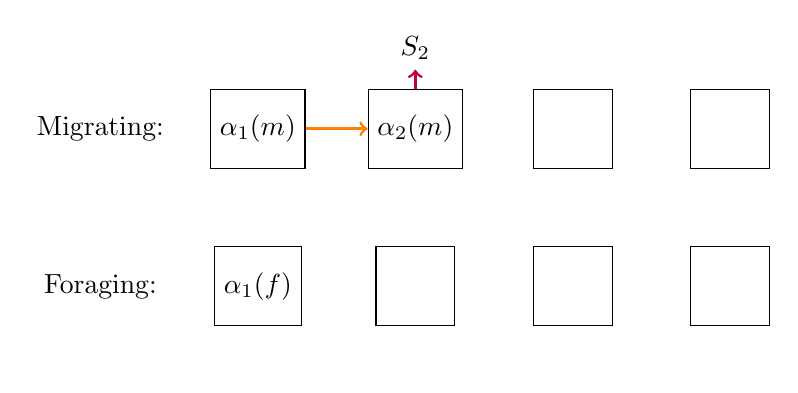
\begin{tikzpicture}[node distance=2cm, block/.style={draw, minimum width=1cm, minimum height=1cm}]

  % First row
  \node[block] (A1) {$\alpha_1(m)$};
  \node[block, right of=A1] (A2) {$\alpha_2(m)$};
  \node[block, right of=A2] (A3) {};
  \node[block, right of=A3] (A4) {};

  % Second row
  \node[block, below of=A1] (B1) {$\alpha_1(f)$};
  \node[block, right of=B1] (B2) {};
  \node[block, right of=B2] (B3) {};
  \node[block, right of=B3] (B4) {};

  % Labels
  \node[coordinate, left of=A1] (J1) {};
  \node[] at (J1) {Migrating:};
  \node[coordinate, left of=B1] (J2) {};
  \node[] at (J2) {Foraging:};

  \node[coordinate, above of=A1, yshift=-1.25cm] (G1) {};
  \node[above] at (G1) {};
  \node[coordinate, above of=A2, yshift=-1.25cm] (G2) {};
  \node[above] at (G2) {$S_2$};
  \node[coordinate, above of=A3, yshift=-1.25cm] (G3) {};
  \node[above] at (G3) {};
  \node[coordinate, above of=A4, yshift=-1.25cm] (G4) {};
  \node[above] at (G4) {};
  \node[coordinate, below of=B1, yshift=1.25cm] (H1) {};
  \node[below] at (H1) {};
  \node[coordinate, below of=B2, yshift=1.25cm] (H2) {};
  \node[below] at (H2) {};
  \node[coordinate, below of=B3, yshift=1.25cm] (H3) {};
  \node[below] at (H3) {};
  \node[coordinate, below of=B4, yshift=1.25cm] (H4) {};
  \node[below] at (H4) {};

  % Horizontal arrows
  \draw[->, line width=1pt, opacity=1, color=orange] (A1.east) -- (A2.west);
  \draw[->, line width=1pt, opacity=0] (A2.east) -- (A3.west);
  \draw[->, line width=1pt, opacity=0] (A3.east) -- (A4.west);
  \draw[->, line width=1pt, opacity=0] (B1.east) -- (B2.west);
  \draw[->, line width=1pt, opacity=0] (B2.east) -- (B3.west);
  \draw[->, line width=1pt, opacity=0] (B3.east) -- (B4.west);

  % diagonal to blocks
  \draw[->, line width=1pt, opacity=0] (A1.south east) -- (B2.north);
  \draw[->, line width=1pt, opacity=0] (A2.south east) -- (B3.north);
  \draw[->, line width=1pt, opacity=0] (A3.south east) -- (B4.north);
  \draw[->, line width=1pt, opacity=0,color=blue] (B1.north east) -- (A2.south west);
  \draw[->, line width=1pt, opacity=0] (B2.north east) -- (A3.south);
  \draw[->, line width=1pt, opacity=0] (B3.north east) -- (A4.south);

  % vertical arrow
  \draw[->, line width=1pt, opacity=1, color=purple] (A2.north) -- (G2.south);


\end{tikzpicture}
\end{center}

where: 
\begin{equation}
    \begin{aligned}
    \alpha_2(m) = \textcolor{orange}{p(X_2=m | X_1=m) \alpha_{1}(m)}\times \textcolor{purple}{p(S_2 | X_2 = m)}.
    \end{aligned}
\end{equation}
    
\end{frame}

\begin{frame}
\frametitle{Modifying forward algorithm: suppose foraging $\rightarrow$ migrating not possible}


\begin{center}
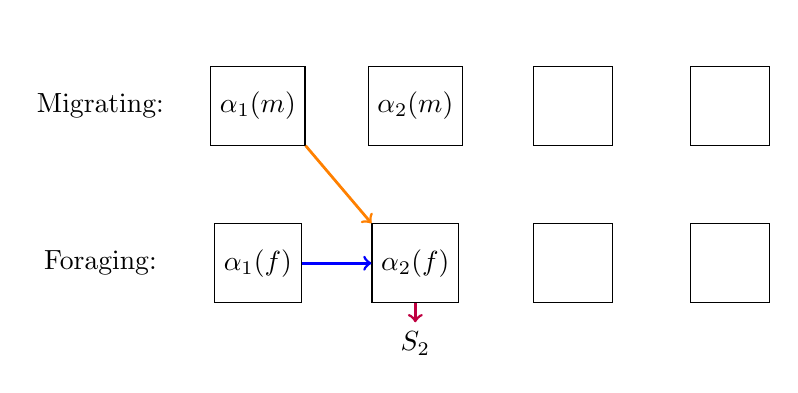
\begin{tikzpicture}[node distance=2cm, block/.style={draw, minimum width=1cm, minimum height=1cm}]

  % First row
  \node[block] (A1) {$\alpha_1(m)$};
  \node[block, right of=A1] (A2) {$\alpha_2(m)$};
  \node[block, right of=A2] (A3) {};
  \node[block, right of=A3] (A4) {};

  % Second row
  \node[block, below of=A1] (B1) {$\alpha_1(f)$};
  \node[block, right of=B1] (B2) {$\alpha_2(f)$};
  \node[block, right of=B2] (B3) {};
  \node[block, right of=B3] (B4) {};

  % Labels
  \node[coordinate, left of=A1] (J1) {};
  \node[] at (J1) {Migrating:};
  \node[coordinate, left of=B1] (J2) {};
  \node[] at (J2) {Foraging:};

  \node[coordinate, above of=A1, yshift=-1.25cm] (G1) {};
  \node[above] at (G1) {};
  \node[coordinate, above of=A2, yshift=-1.25cm] (G2) {};
  \node[above] at (G2) {};
  \node[coordinate, above of=A3, yshift=-1.25cm] (G3) {};
  \node[above] at (G3) {};
  \node[coordinate, above of=A4, yshift=-1.25cm] (G4) {};
  \node[above] at (G4) {};
  \node[coordinate, below of=B1, yshift=1.25cm] (H1) {};
  \node[below] at (H1) {};
  \node[coordinate, below of=B2, yshift=1.25cm] (H2) {};
  \node[below] at (H2) {$S_2$};
  \node[coordinate, below of=B3, yshift=1.25cm] (H3) {};
  \node[below] at (H3) {};
  \node[coordinate, below of=B4, yshift=1.25cm] (H4) {};
  \node[below] at (H4) {};

  % Horizontal arrows
  \draw[->, line width=1pt, opacity=0] (A1.east) -- (A2.west);
  \draw[->, line width=1pt, opacity=0] (A2.east) -- (A3.west);
  \draw[->, line width=1pt, opacity=0] (A3.east) -- (A4.west);
  \draw[->, line width=1pt, opacity=1,color=blue] (B1.east) -- (B2.west);
  \draw[->, line width=1pt, opacity=0] (B2.east) -- (B3.west);
  \draw[->, line width=1pt, opacity=0] (B3.east) -- (B4.west);

  % diagonal to blocks
  \draw[->, line width=1pt, opacity=1,color=orange] (A1.south east) -- (B2.north west);
  \draw[->, line width=1pt, opacity=0] (A2.south east) -- (B3.north);
  \draw[->, line width=1pt, opacity=0] (A3.south east) -- (B4.north);
  \draw[->, line width=1pt, opacity=0] (B1.north east) -- (A2.south west);
  \draw[->, line width=1pt, opacity=0] (B2.north east) -- (A3.south);
  \draw[->, line width=1pt, opacity=0] (B3.north east) -- (A4.south);

  % vertical arrow
  \draw[->, line width=1pt, opacity=1, color=purple] (B2.south) -- (H2.north);

\end{tikzpicture}
\end{center}

where: 
\begin{equation}
    \begin{aligned}
    \alpha_2(f) = \{&\textcolor{orange}{p(X_2=f | X_1=m) \alpha_{1}(m)} +\textcolor{blue}{p(X_2=f | X_1=f) \alpha_{1}(f)}\}\\
    &\times \textcolor{purple}{p(S_2| X_2 = f)} 
    \end{aligned}
\end{equation}
    
\end{frame}

\begin{frame}
\frametitle{Elephants revisited}

\begin{figure}
    \centering
    \includegraphics[width=0.6\textwidth]{figures/elephant_parturition.jpg}
\end{figure}

We assumed that log-mean daily speed follows:
%
\begin{equation*}
    S_t|X_t \sim \text{normal}(\mu_{X_t}, \sigma),
\end{equation*}
%
where $\mu_{\text{pre}} \& \mu_{\text{post}} \sim \text{normal}(-1, 0.5)$ and $\mu_{\text{parturition}} \sim \text{normal}(-1.5, 0.5)$.

\end{frame}

\begin{frame}
\frametitle{Estimates of parturition dates and states: Flaubert}

\begin{figure}
    \centering
    \includegraphics[width=1\textwidth]{figures/flaubert.png}
\end{figure}
    
\end{frame}


\begin{frame}
\frametitle{Estimates of parturition dates and states: Aztec}

\begin{figure}
    \centering
    \includegraphics[width=1\textwidth]{figures/aztec.png}
\end{figure}
    
\end{frame}

\end{document}